\documentclass{article}
\usepackage[utf8]{inputenc}
\usepackage[english]{babel}
\usepackage{fullpage,amsmath,amssymb,graphics, graphicx,enumitem,ulem,parskip,xcolor}

\title{CSC311 Final Project}
\author{Jia Lin Yuan, Steven Tran, Luyang Shang}
\date{December 15, 2020}

\begin{document}
\maketitle
\section{Part A}
\begin{enumerate}[label=\arabic*.]
    \item For this approach, we use the KNN algorithm to impute the missing values.
        \begin{enumerate}[label=(\alph*)]
            \item See \texttt{knn.py} for the supporting code. For distance by user, we have:

                \noindent
                \begin{minipage}{0.5\linewidth}
                    \centering
                    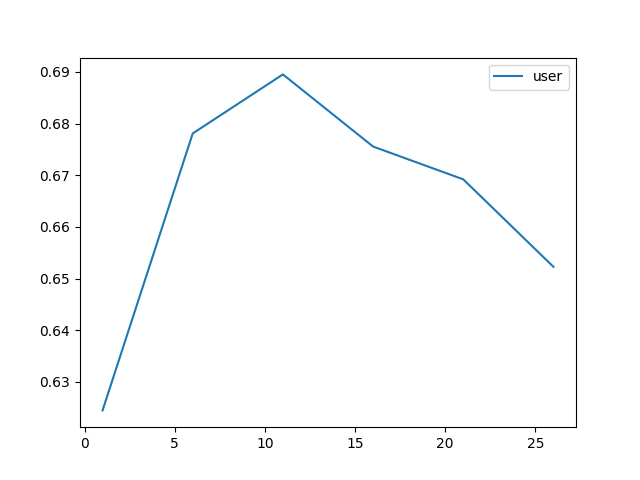
\includegraphics[width=\linewidth]{../starter_code/figs/knn_user.png}
                \end{minipage}\hfill
                \begin{minipage}{0.5\linewidth}
                    \center
                    \begin{tabular}{c|c}
                        $k$ & Validation Accuracy \\\hline
                        1 & 0.6244707874682472\\
                        6 & 0.6780976573525261\\
                        11 & 0.6895286480383855\\
                        16 & 0.6755574372001129\\
                        21 & 0.6692068868190799\\
                        26 & 0.6522720858029918
                    \end{tabular}
                \end{minipage}
            \item The best value of $k$ for user-based collaborative filtering is $k^*=11$.
            \item For distance by item, we have:

                \noindent
                \begin{minipage}{0.5\linewidth}
                    \centering
                    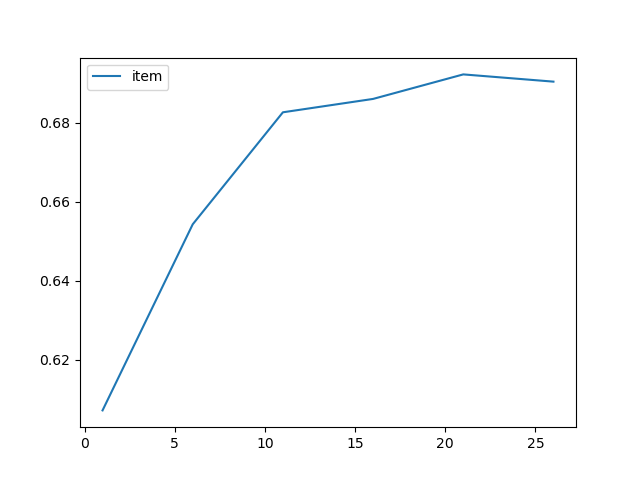
\includegraphics[width=\linewidth]{../starter_code/figs/knn_item.png}
                \end{minipage}\hfill
                \begin{minipage}{0.5\linewidth}
                    \center
                    \begin{tabular}{c|c}
                        $k$ & Validation Accuracy \\\hline
                        1 & 0.607112616426757\\
                        6 & 0.6542478125882021\\
                        11 & 0.6826136042901496\\
                        16 & 0.6860005644933672\\
                        21 & 0.6922099915325995\\
                        26 & 0.69037538808919
                    \end{tabular}
                \end{minipage}
                And the best value of $k$ for item-based collaborative filtering is $k^*=21$.
            \item For the chosen values of $k$: $k^*_{\text{user}}=11$, $k^*_{\text{item}}=21$, we find that the test accuracy is 0.68416596105 and 0.68165274090, respectively. 
                \textcolor{red}{TODO: KNN for user has better test accuracy than item, Alan}
            \item Here are two limitations of KNN for this task:
                \begin{itemize}
                    \item KNN is slow. Even with only 542 items and 1774 users it takes a while to predict.
                    \item Using Euclidean distance, we consider distances in all dimension to be equal. For example if A and B's math skills are very different but english, physics, and other subjects are similar, the KNN will still predict A's math question similar to B's math questions (since skill in math is treated equally with other subjects).
                \end{itemize}

        \end{enumerate}
        
    \item In this approach, we use Item Response Theory to predict students' correctness to diagnostic questions.
        \begin{enumerate}[label=(\alph*)]
            \item 
            \item 
            \item 
            \item 
        \end{enumerate}
        
    \item In this approach, we use both matrix factorization and neural networks.
        \begin{enumerate}[label=(\roman*)]
            \item Matrix Factorization \textcolor{red}{remove this if we are not using it}
                \begin{enumerate}[label=(\alph*)]
                    \item d
                \end{enumerate}
            \item Neural Networks
                \begin{enumerate}[label=(\alph*)]
                    \item \textcolor{red}{Not sure what this is asking.}
                    \item See \texttt{neural\_network.py}
                    \item We trained models using a variety of hyperparameters and found that the best combinations were:
                    \begin{center}
                        \begin{tabular}{c|c|c|c|c|c}
                            $k$ (latent dim.) & learning rate & epochs & $\lambda$ (penalty) & train cost & val. accuracy \\\hline
                            10 & 0.01 & 100 & 0.1 & 10545.283 & 0.68784 \\
                            10 & 0.01 & 100 & 0.5 & 19321.324219 & 0.69038 \\
                            50 & 0.05 & 10  & 0.5 & 17700.197 & 0.690799 \\
                            100 & 0.01 & 50 & 0.1 & 7667.879 & 0.68246 \\
                            100 & 0.05 & 10 & 0 & 6923.447 & 0.68346 \\
                            200 & 0.01 & 50 & 0.1 & 6638.1338 & 0.6782388 \\
                            200 & 0.01 & 50 & 0.5 & 16577.74 & 0.6745696 
                        \end{tabular}
                    \end{center}
                    Setting $k=500$ led to comparatively low validation accuracy (mean average of $0.651150$). For the other values of $k$, there weren't discernible correlations between the choice of hyperparameters and the performance of the model; the lower training cost and higher validation accuracy can probably be attributed to luck. We choose $k^*=10$ since the combination on the second row has a validation accuracy of 0.69038.
                \item d
                \end{enumerate}
        \end{enumerate}
\end{enumerate}
\section{Part B}
\begin{enumerate}[label=\arabic*.]
    \item d
    \item d
    \item d
    \item d
\end{enumerate}
\end{document}
